\section{Methodology}
This project applies reinforcement learning to control the architecture of a quantum circuit during training. The methodology below covers the machine-learning side (data, model, evaluation protocol) and the reinforcement-learning side (environment, agent, reward) of the system.

\begin{figure}[htbp]
\centering
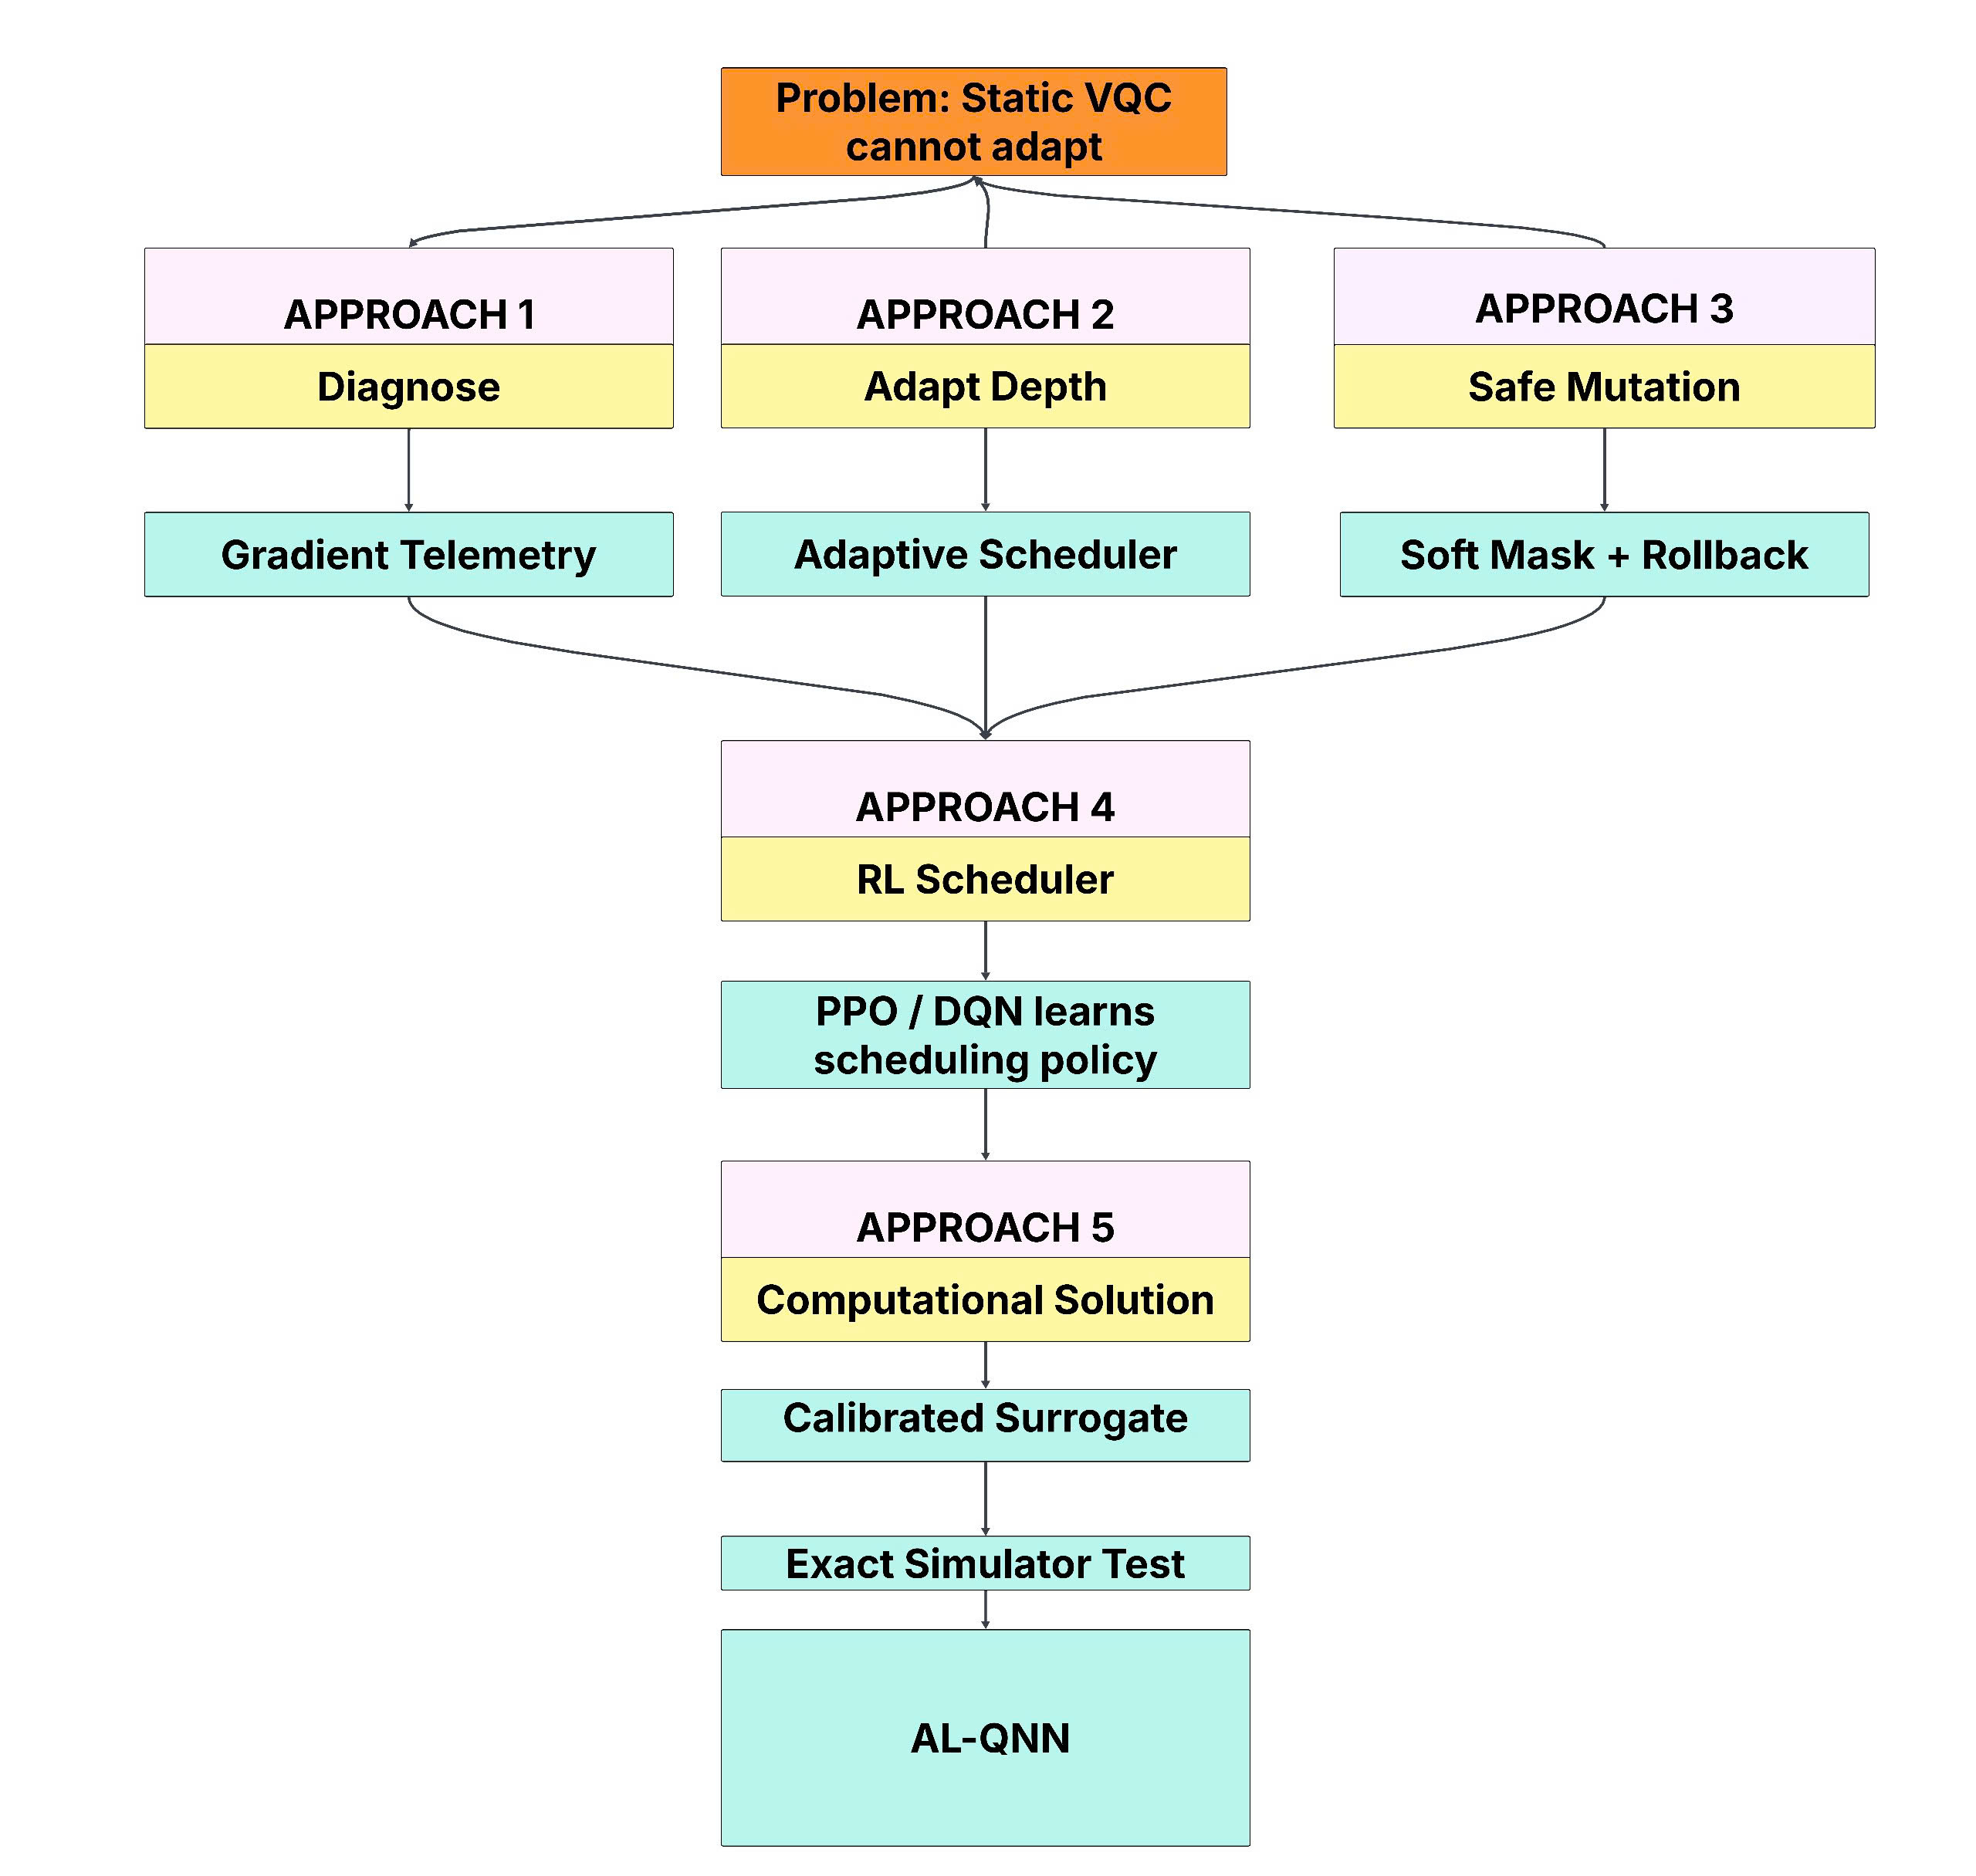
\includegraphics[width=0.7\textwidth]{figure/fig_solution_approach.jpg}
\caption{From problem to solution. A static VQC cannot adapt (top); Approaches 1--3 diagnose circuit health via gradient telemetry (Section~4.4.1), adapt depth via a scheduler (Section~4.4.2), and apply changes through safe, reversible mutation (Section~4.4.3); Approach~4 learns this diagnose-adapt-mutate policy end-to-end with PPO/DQN (Section~4.4.4); and Approach~5 makes that learning computationally tractable by training on a calibrated surrogate before evaluating on an exact PennyLane simulator (Section~4.4.5) -- together defining AL-QNN.}
\label{fig:solution_approach}
\end{figure}

\subsection{Research Questions and Objectives}

\subsubsection{Research Questions}
The project addresses three research questions. RQ1: can a variational quantum classifier built from a hardware-efficient ansatz reach competitive accuracy on real tabular datasets at NISQ-scale qubit counts? RQ2: to what extent does the barren plateau limit trainability at these scales, and how does that limit depend on the cost function and the circuit depth? RQ3: does scheduling the circuit depth (rather than fixing it) improve or at least match a well-tuned fixed-depth model?

\subsubsection{Project Objectives}
The objective is to build the classifier, measure the barren plateau empirically, and evaluate performance under a consistent, leakage-free protocol.

\subsection{Data}

\subsubsection{Dataset Collection Overview}
The project data package contains several binary-classification tabular datasets spanning healthcare, finance, and industrial maintenance. This section covers only the datasets for which a scheduler-comparison run was actually logged and reported in Section~6 (\Cref{tab:datasets}); the loader also supports a few additional datasets (a high-dimensional image case and a small clean benchmark) that were used only for earlier smoke-testing and preprocessing checks and never carried through to a logged comparison run, and are therefore left out of this report entirely rather than described without matching results. Dataset facts below (native instance and feature counts, provenance) are attributed to the original dataset authors or their UCI Machine Learning Repository records; project-specific sample counts, feature selection, class balancing, and encoding steps are attributed to the AL-QNN project's data-preparation scripts and loader (\texttt{data/prepare\_*.py}, \texttt{scripts/dataset.py}).

\subsubsection{Common Data Preparation Pipeline}
Preprocessing is deterministic and strictly fit on the training split to prevent leakage. The project loader converts each dataset to a binary target, then applies a fixed-seed stratified split into train, validation, and test; a Z-score standardization is fitted on the training split and applied to all splits; the feature count is then reconciled with the requested qubit count in one of three ways -- principal-component analysis (PCA), fitted on the training data, when the native feature count exceeds the qubit count; a direct one-to-one mapping when the two are equal; or zero-padding with constant, uninformative columns when the native feature count is smaller than the requested qubit count -- and finally every feature is rescaled to the angle-encoding range [0, π]. None of the five datasets reported in Section~6 currently needs the zero-padding case at their evaluated qubit count; it remains a supported loader behaviour for a dataset whose native feature count is smaller than the requested qubit count, kept honest here rather than described as if exercised. Missing values (for example in the Heart dataset) are removed before splitting. Several datasets are also balanced to an even class ratio by undersampling the majority class, which makes scheduler comparisons less dependent on class imbalance but means the processed files should not be read as representative of the original class distributions; AI4I is the one exception to undersampling (Section~4.2, AI4I 2020 Predictive Maintenance). This end-to-end flow runs from the raw per-dataset CSV to the angle-encoded input consumed by the hardware-efficient ansatz of Section~4.4.2, and this final $[0,\pi]$ encoding step is shared by all five datasets below, not just AI4I.

\begin{figure}[htbp]
\centering
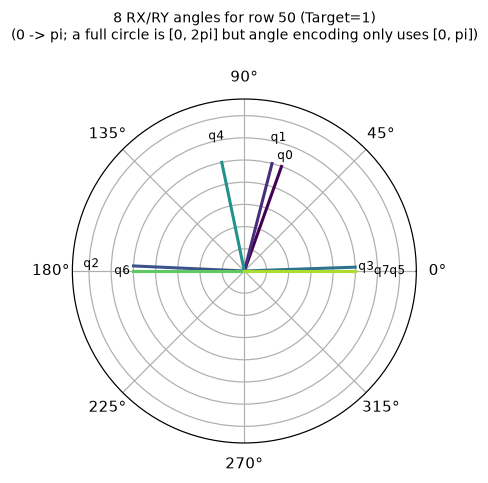
\includegraphics[width=0.55\textwidth]{figure/output.png}
\caption{A worked example of the final angle-encoding step every dataset in \Cref{tab:datasets} goes through: the eight $R_X$/$R_Y$ rotation angles produced by encoding a single training row (an AI4I failure case, shown here as a concrete instance), plotted on $[0,\pi]$ of a polar axis to show that no encoded angle exceeds the half-circle the ansatz actually uses.}
\label{fig:angle_example}
\end{figure}

\FloatBarrier
\subsubsection{Pima Indians Diabetes}
The Pima Indians Diabetes dataset records 768 observations of women of Pima Indian heritage, at least 21 years old, with eight predictive variables covering pregnancies, glucose, blood pressure, skin thickness, insulin, BMI, diabetes pedigree function, and age; the original class split is imbalanced at 268 positive versus 500 negative cases \citep{smith1988pima}. The project's preparation script balances the classes to 536 observations (268 per class) and retains all eight original predictive variables without PCA, since eight features already matches the eight-qubit target register. This gives a direct 8-feature-to-8-qubit mapping, making Pima useful for isolating the effect of circuit depth and adaptive scheduling from any dimensionality-reduction confound; it contributes one of the supplementary single-seed deployments reported in \Cref{tab:pima} (Section~6.1).

\subsubsection{Heart Disease -- Cleveland}
The UCI Cleveland Heart Disease record describes 303 instances and 13 predictive attributes -- age, sex, chest-pain type, resting blood pressure, cholesterol, fasting blood sugar, resting ECG, maximum heart rate, exercise-induced angina, ST depression, slope, number of major vessels, and thalassemia -- with an original five-level target that is conventionally binarized to absence (0) versus presence (1--4) of disease \citep{detrano1989heart}. The project's preparation script follows this binary convention, removes rows with missing values, balances the resulting classes, and applies \texttt{SelectKBest} with an ANOVA F-test to reduce 13 features to the 8 most informative ones, yielding 274 processed observations (137 per class). This dataset is used both for the AI4I-style barren-plateau characterization and, later, for the real PennyLane deployment reported in \Cref{tab:heart}.

\subsubsection{Parkinson's -- Oxford Parkinson's Disease Detection Dataset}
The UCI Parkinsons record uses biomedical voice measurements -- fundamental-frequency measures, jitter, shimmer, noise-to-harmonics ratios, and nonlinear dynamical measures -- drawn from 195 voice recordings of 31 people (23 with Parkinson's disease), reported as 197 instances over 22 features \citep{little2007parkinsons}. The project's preparation script selects 8 features from the original 22 with \texttt{SelectKBest} and balances the classes to a 96-observation set (48 per class). Its small sample size makes this dataset useful for probing scheduler stability under sensitivity to the train/validation split and random seed, and it contributes one of the supplementary single-seed deployments reported in \Cref{tab:parkinsons} (Section~6.1).

\subsubsection{Statlog German Credit}
The Statlog German Credit dataset contains 1,000 instances and 20 categorical and integer attributes describing applicants as good or bad credit risks \citep{hofmann1994german}. The project's preparation script converts categorical values to numerical category codes, binarizes the credit-risk label, balances the classes to 600 observations (300 per class), and selects 8 features from the original 20 with \texttt{SelectKBest}, producing a file directly compatible with an eight-qubit input representation. A Logistic Regression cross-validation sanity check on the processed file reports approximately 0.725 accuracy, which the project treats as a moderate classification difficulty suitable for scheduler comparison; German Credit is accordingly used for one of the supplementary single-seed scheduler-comparison deployments reported alongside AI4I and Heart Disease in \Cref{tab:german} (Section~6.1).

\subsubsection{AI4I 2020 Predictive Maintenance}
The AI4I 2020 Predictive Maintenance dataset is a synthetic industrial dataset of 10,000 observations, multivariate and time-series in nature, whose binary machine-failure label is set to 1 when at least one of several defined failure modes occurs \citep{matzka2020ai4i}. The project representation combines five numerical process/sensor variables with the three one-hot-encoded categories of the machine \texttt{Type} field to produce a fixed 8-column engineered input. The raw label is strongly imbalanced (9,661 non-failure vs 339 failure, $\approx$3.4\% positive); the loader preserves this natural ratio when reading the data, stratified-subsampling only if a smaller \texttt{max\_samples} budget is requested, rather than discarding real majority-class rows just to force balance. Class balance is instead restored by SMOTE \citep{chawla2002smote}, applied only to the training split, only after the train/validation/test split and after the one-to-one feature mapping and $[0,\pi]$ angle-encoding scaling described below -- so synthetic points are interpolated in the same already-encoded space the ansatz consumes, and the validation and test splits are left at the true $\approx$3.4\% ratio for an honest evaluation. This fixed 8-column representation maps one-to-one onto the project's 8-qubit scope (Section~1.6), the same direct mapping as Pima, so the primary result table (\Cref{tab:ai4i}, three seeds, $n=8$) runs on 8 real, independently informative features with no dimensionality reduction or padding involved. AI4I is nonetheless the project's primary dataset, chosen in part because it tests whether a scheduler remains effective under an application domain with severe native class imbalance and multiple physical operating variables, rather than only on small, already-clean academic benchmarks.

\begin{figure}[htbp]
\centering
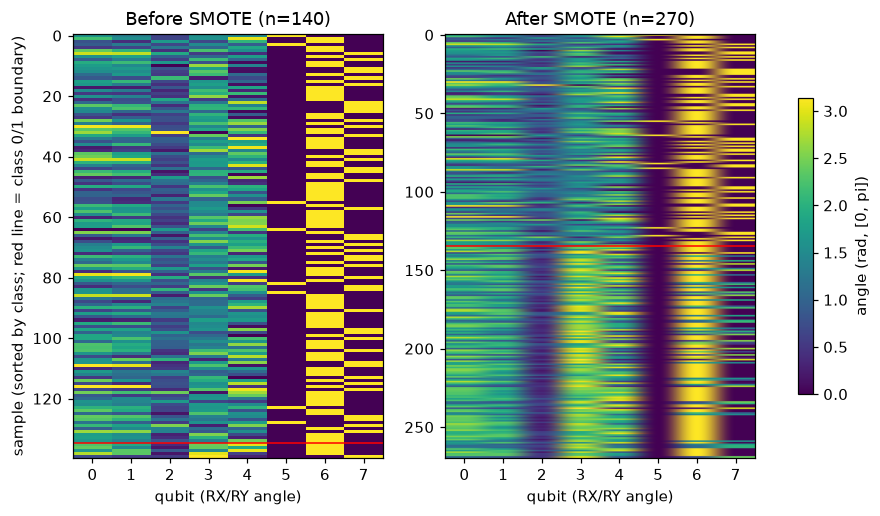
\includegraphics[width=0.95\textwidth]{figure/before_vs_after_SMOTE.png}
\caption{A representative training-split subset's angle-encoded features (one column per qubit) before and after SMOTE, samples sorted by class with the class-0/1 boundary marked in red. Every value stays inside $[0,\pi]$ because SMOTE interpolates directly in the already fit-and-scaled encoding space (Section~4.2), not in raw feature space.}
\label{fig:smote_angles}
\end{figure}

\begin{figure}[htbp]
\centering
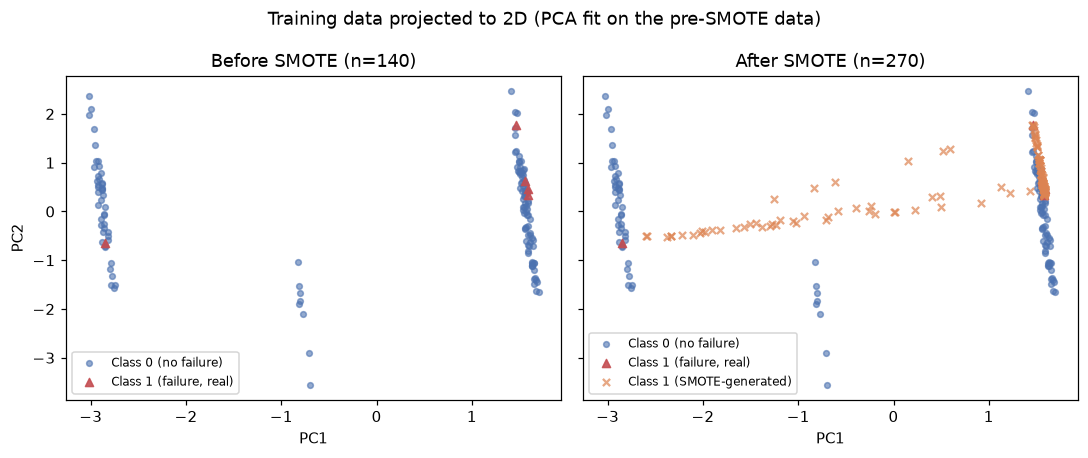
\includegraphics[width=0.85\textwidth]{figure/smott.png}
\caption{The same training-split subset projected onto its first two principal components (PCA fit on the pre-SMOTE data, for visualization only -- AI4I itself uses no PCA at $n=8$, per \Cref{tab:datasets}). SMOTE-generated failure samples (orange) interpolate between the real failure samples (red) rather than forming an unrelated cluster, which is the qualitative check this figure exists to make.}
\label{fig:smote_pca}
\end{figure}


\begin{table}[htbp]
\centering
\caption{Datasets used, their native feature count, and the qubit-count/feature-reduction mapping applied.}
\label{tab:datasets}
\begin{tabular}{|p{3.4cm}|p{2.6cm}|p{2.2cm}|p{4.6cm}|}
\hline
\textbf{Dataset} & \textbf{Native features} & \textbf{Qubits used} & \textbf{Reduction applied} \\
\hline
AI4I 2020 (predictive maintenance) & 8 (fixed: 5 numeric + 3 one-hot) & 8 & None -- one-to-one mapping \\
Heart Disease (Cleveland) & 13 & 8 & Univariate feature selection, 13 to 8 \\
Parkinson's & 22 & 8 & Univariate feature selection, 22 to 8 \\
Pima Diabetes & 8 & 8 & None -- one-to-one mapping \\
German Credit (Statlog) & 20 & 8 & Univariate feature selection, 20 to 8 \\
\hline
\end{tabular}
\end{table}

\subsubsection{Dataset Suitability and Usage Across Experiments}
AI4I 2020 predictive maintenance is the primary dataset (\Cref{tab:ai4i}, three seeds) and Heart Disease is the dataset behind the primary real PennyLane deployment (\Cref{tab:heart}); together these anchor the core evaluation design of Section~6.1--6.2. German Credit, Parkinson's, and Pima each contribute one additional single-seed PennyLane deployment, reported as supplementary evidence in \Cref{tab:german,tab:parkinsons,tab:pima} (Section~6.1) rather than as part of the core design itself. Taken together, the five datasets kept in this report are deliberately heterogeneous: Pima and Heart give, respectively, a direct feature-to-qubit case and a feature-selection case on real medical data; Parkinson's stresses scheduler stability on a small sample; and German Credit and AI4I supply moderate-difficulty financial and severely-imbalanced industrial benchmarks. A scheduler that only performs well on one simple dataset would not be expected to generalize across this range of sample size, class balance, and preprocessing requirements, which is why Section~6 draws its regimes and supplementary checks from more than one of these sources rather than reporting a single dataset's results.

\subsection{Feature Selection and Engineering}

\subsubsection{Feature-to-Qubit Mapping}
The number of input features is matched to the qubit count. Where a dataset already has exactly as many informative features as qubits -- Pima and AI4I with eight features each for eight qubits -- the mapping is one-to-one and no dimensionality reduction is applied, preserving all information. Where there are more features than qubits, the dimension is reduced by univariate feature selection via \texttt{SelectKBest} (Heart, 13 $\rightarrow$ 8; Parkinson's, 22 $\rightarrow$ 8; German Credit, 20 $\rightarrow$ 8); none of the five datasets reported in Section~6 currently needs PCA or zero-padding at their evaluated qubit count, though the loader supports both (Section~4.2, Common Data Preparation Pipeline) and PCA remains the intended route for a higher-dimensional or less individually-interpretable feature set, such as the image and small-benchmark cases mentioned in Section~4.2 that were used only for smoke-testing. Each selected feature is then engineered into a rotation angle in [0, π] by angle encoding.

\subsubsection{Choice of Reduction Strategy}
Univariate selection is used for every dataset in this report that needs reduction at all -- Heart, Parkinson's, and German Credit -- because their raw features are already individually interpretable clinical, demographic, or financial measurements, so discarding the least informative ones preserves the meaning of the remaining features and keeps the angle-encoding mapping interpretable feature-by-feature. PCA was used in an earlier, wider-qubit-range version of this project for AI4I's fixed, sensor-derived feature set; at the project's current 8-qubit scope AI4I's 8 native features map one-to-one onto 8 qubits instead (Section~4.2, AI4I 2020 Predictive Maintenance), so no dataset currently reported in Section~6 exercises the PCA path, though it remains available for a higher-dimensional or less individually-interpretable feature set should one be added. Both reduction strategies converge on the same downstream representation -- exactly \$n\$ real-valued features per sample, rescaled to [0, π] -- so that the ansatz and the RL environment never need to know which reduction strategy produced their input: Z-score standardization reshapes each raw feature's distribution, PCA or \texttt{SelectKBest} reduce $n$ raw features down to $k$ qubit features, and the resulting $k$-dimensional vector is rescaled into $[0,\pi]$ and loaded as a per-qubit $R_Y(\theta_i)$ rotation.

\subsection{Approach Overview: Diagnose, Adapt, Mutate Safely}
\quad Five coupled sub-problems must be solved for a scheduler to safely and practically control circuit depth: diagnosing the circuit's true state (Approach~1), deciding what structural change that state calls for (Approach~2), applying any change without risking the run (Approach~3), learning the diagnose-to-action mapping end-to-end rather than hand-coding it (Approach~4), and making that learning loop computationally tractable in the first place (Approach~5). \Cref{fig:solution_approach} at the start of this chapter traces exactly this chain from problem to the finished AL-QNN system; the five subsections below introduce each briefly, with full technical detail in Section~4.4.2 (circuit model) and Section~4.7 (environment, agent, reward). \Cref{tab:approach_io} summarizes what each approach consumes and produces, so the chain from raw telemetry to a deployed policy can be followed at a glance before the detail.

\begin{table}[htbp]
\centering
\caption{Input and output of each approach.}
\label{tab:approach_io}
\begin{tabular}{|p{2.6cm}|p{5.3cm}|p{5.3cm}|}
\hline
\textbf{Approach} & \textbf{Input} & \textbf{Output} \\
\hline
1: Diagnosis & Five raw runtime signals per epoch; offline Stage~1C risk table & One of five diagnosis labels -- logged (Appendix~B), fed into the state (\Cref{tab:state}), gates $w_1$ (\Cref{tab:reward}) \\
2: Scheduling & Diagnosis label (Approach~1); current depth and depth cap & Masked space of legal actions from \Cref{tab:actions} \\
3: Safe Mutation & Agent-selected structural action (Approach~4); checkpointed parameters & Committed circuit (gates removed) or rolled-back circuit (checkpoint restored) \\
4: RL Scheduler & Sixteen-dimensional telemetry state (\Cref{tab:state}) & One selected action from \Cref{tab:actions}, trained on the reward of \Cref{tab:reward} \\
5: Computational Solution & Stage~1 barren-plateau measurements & Trained policy, deployed and evaluated on PennyLane (Section~6) \\
\hline
\end{tabular}
\end{table}

\subsubsection{Approach 1: Multi-Dimensional Gradient Telemetry and Diagnosis}
A naive rule -- flag a barren plateau whenever the gradient norm drops below a threshold -- cannot tell a true plateau apart from ordinary behaviour that looks the same: convergence, a local minimum, one dead layer amid otherwise healthy ones, or plain shot noise. Approach~1 instead diagnoses the circuit every epoch from five raw runtime signals $\mathbf{s} \in \mathbb{R}^5$, mapped to continuous risk probabilities by a sigmoid,
\begin{equation}
p_k = \sigma(s_k) = \frac{1}{1+e^{-s_k}}, \qquad k = 1,\dots,5,
\end{equation}
and checked against the offline risk table calibrated in Stage~1C from the Stage~1 barren-plateau measurements (Section~4.7.1). A fixed priority order resolves these probabilities into exactly one label: \textbf{solved/converged} (loss at target -- locks out further mutation), \textbf{local minimum} (loss flat, gradient still non-trivial -- keep optimizing), \textbf{dead layer} (one layer's gradient collapsed, rest healthy -- mask that layer only), \textbf{ambiguous} (inconclusive -- watch, don't act), or \textbf{true barren plateau} (every layer collapsed under high structural risk -- lock depth growth). The label is logged every epoch (\texttt{is\_solved}, \texttt{is\_converged}, \texttt{is\_local\_min}, \texttt{is\_dead\_layer}, \texttt{is\_ambiguous}, \texttt{is\_true\_bp}, Appendix~B), feeds the agent's sixteen-dimensional state (\Cref{tab:state}), and gates the reward directly: once solved, the gradient-variance weight ($w_1$ in \Cref{tab:reward}) is forced toward zero so the agent cannot keep collecting reward by disturbing a converged model.

\subsubsection{Approach 2: Adaptive Circuit Scheduling}
Once the circuit's state is known, the question becomes what to do about it. Each layer $\ell$ of the ansatz follows the hardware-efficient ansatz pattern of \citet{kandala2017hardware}: a single-qubit rotation block on every qubit followed by a fixed entangling layer. Concretely, each layer applies, to every qubit $i \in \{1, \dots, n\}$, the single-qubit Euler decomposition
\begin{equation}
U_i^{(\ell)}(\theta) = R_Z(\theta_{i,3}^{(\ell)})\, R_Y(\theta_{i,2}^{(\ell)})\, R_Z(\theta_{i,1}^{(\ell)})
\end{equation}
followed by a fixed nearest-neighbour entangling layer $\mathrm{CNOT}_{i,i+1}$ applied for $i = 1, \dots, n-1$. A depth-$d$ circuit is then the ordered product
\begin{equation}
U(\theta) = \prod_{\ell=1}^{d} \left( \prod_{i=1}^{n-1} \mathrm{CNOT}_{i,i+1} \right) \left( \bigotimes_{i=1}^{n} U_i^{(\ell)}(\theta) \right)
\end{equation}
acting on the angle-encoded input state, with the classification output read from a measurement of the final state. The global cost used in Section~1.4's problem statement is a function of the full $n$-qubit measurement outcome, whereas the local cost this project targets restricts each cost term to a small subset of qubits (following the construction of \citet{cerezo2021cost}); this is what weakens the exponential qubit-count scaling of the gradient variance into the depth-dependent behaviour exploited by the scheduler throughout Section~6.

This ansatz was chosen because it is expressive, respects device connectivity, and keeps circuits shallow -- the properties required on NISQ hardware. At 8 qubits each layer contributes 24 trainable parameters (8 qubits $\times$ 3 rotations); the circuit therefore holds 24$\times$depth parameters, e.g. 48 at depth 2 and 120 at depth 5. The depth is bounded by a cap (typically 6-16 depending on the qubit count).

A static hardware-efficient ansatz fixes $D(t) = D_{\text{fixed}}$ for every epoch $t$; Approach~2 instead makes depth $D(t)$ a variable the agent controls through the five discrete actions of \Cref{tab:actions} -- adding a layer when expressivity is needed and gradients are healthy, holding while the optimizer converges, stopping growth once Approach~1 flags solved or true-barren-plateau risk, and proposing to prune a layer or reduce entanglement when only part of the circuit is diagnosed as harmful. An action mask, rebuilt each epoch from the current depth, the depth cap, and the diagnosis state, removes illegal or unsafe actions before the agent ever selects among them (Section~4.7.2), so the learned policy always stays inside hardware-consistent bounds.

\subsubsection{Approach 3: Safe Mutation via Soft-Masking and Registry Rollback}
A structural change proposed under Approach~2 might hurt training, so no mutation is ever applied irreversibly. A layer proposed for pruning or entanglement reduction is first soft-masked rather than deleted: a coefficient $S(t)$ scales its contribution and decays over a short window of $T$ epochs (5 by default) on a cosine schedule \citep{loshchilov2017sgdr},
\begin{equation}
S(t) = \tfrac{1}{2}\bigl[1+\cos(\pi t / T)\bigr], \qquad t = 0,\dots,T,
\end{equation}
chosen because $\mathrm{d}S/\mathrm{d}t = 0$ at both endpoints, so masking introduces no abrupt jump that would desynchronize the Adam optimizer's momentum buffers. The circuit's parameters are checkpointed in a parameter registry before masking begins; at the end of the window the mutation is \textbf{committed} (gates permanently removed) if the worst loss reached during the window stayed within tolerance,
\begin{equation}
\frac{\mathcal{L}_{\text{peak}} - \mathcal{L}_{\text{start}}}{\mathcal{L}_{\text{start}}} \;\le\; \delta \quad (\delta = 0.02 \text{ by default}),
\end{equation}
and \textbf{rolled back} to the exact checkpointed state otherwise -- tracking the peak rather than the final-epoch loss so that mid-window damage cannot be hidden by late recovery. Algorithm~1 (Section~4.7.4) formalizes this loop; it is what lets the scheduler explore structural changes -- something a static ansatz can never do -- without risking permanent damage to a run that was already working.

\subsubsection{Approach 4: RL Scheduler}
Approaches 1--3 define what the agent perceives and what it may do, but not how it decides. Approach~4 learns that mapping end-to-end instead of hand-coding it: the sixteen-dimensional telemetry state (\Cref{tab:state}) is fed to a PPO \citep{schulman2017proximal} or DQN \citep{mnih2015human} agent, which outputs one of the five actions of \Cref{tab:actions} every epoch and is trained to maximize the weighted reward of \Cref{tab:reward}. This favours a general-purpose, off-the-shelf algorithm over a hand-designed heuristic (Section~3.5.2): the project's contribution is the state, action, and reward design around the circuit, not a new RL algorithm. Full agent, state, and reward design is given in Section~4.7.2--4.7.4.

\subsubsection{Approach 5: Computational Solution}
Training Approach~4's agent needs millions of environment interactions, but an exact circuit gradient on real quantum hardware requires the parameter-shift rule -- two circuit evaluations per parameter,
\begin{equation}
g_i = \frac{\mathcal{L}(\theta_i + \tfrac{\pi}{2}) - \mathcal{L}(\theta_i - \tfrac{\pi}{2})}{2},
\end{equation}
per \citet{mitarai2018quantum,schuld2019evaluating} -- far too slow to repeat every epoch of every episode. Approach~5 resolves this with the two-simulator design: PPO/DQN train against a fast classical surrogate calibrated on the Stage~1 measurements, while only the final learned policy is deployed and evaluated on PennyLane's exact statevector backend (Section~4.7.1), which obtains the same gradient by backpropagation in a single reverse pass instead of one parameter-shift evaluation at a time. Every number reported in Section~6 comes from this exact-simulator deployment, never from the surrogate alone.

\subsection{Training Configuration}
Training uses exact statevector gradients (backpropagation) on the PennyLane simulator for 40 deployment epochs. Data are split deterministically by a fixed data-split seed (42) into 70\% train and 30\% validation; the deployment and comparison scripts (\texttt{scripts/04\_train\_rl\_scheduler.py}, \texttt{scripts/05\_compare\_schedulers.py}) do not carve out a separate held-out test split for the results in Section~6, so the accuracy, F1, and ROC AUC numbers reported throughout are computed on the validation split -- the same split the scheduler observes every epoch to make its accept/rollback decisions. This is an honestly-reported limitation rather than a leakage bug: no scaler, PCA, or model parameter is ever fit on the validation data, but because the scheduler's structural decisions are themselves conditioned on validation performance, the reported numbers should be read as in-loop validation metrics rather than metrics from data the pipeline never touched. A separate three-way train/validation/test split exists in the shared data loader (\texttt{test\_frac}) and is used by the standalone prediction-export script (\texttt{export\_predictions.py}) that backs the demonstration interface, but it is not the configuration behind either the three-seed AI4I variance check or the single-seed comparison tables in Section~6. AI4I was additionally validated with three random seeds during development (reported as mean $\pm$ standard deviation) to characterize seed variance; the scheduler-comparison tables presented in Section~6 are single-seed and treated as exploratory.

\subsection{Evaluation Metrics}

\subsubsection{Classification and Trainability Metrics}
Classification quality is measured by accuracy, F1 score, and ROC AUC on the validation split (Section~4.5), which is the only non-training split available in the single-seed comparison runs behind Section~6. Trainability is measured by the spatial gradient variance and the near-zero-gradient ratio, which quantify how close the model is to a barren plateau.

\subsubsection{Resource and Scheduler-Behaviour Metrics}
Resource use is measured by the final circuit depth and the number of entangling gates. The scheduler's behaviour is characterized by the number of committed and rolled-back mutations. Metrics from the three-seed AI4I variance check (Section~6.1) are reported as a mean with standard deviation; the scheduler-comparison tables in Section~6 are single-seed.

\subsection{The Reinforcement-Learning Environment}
\subsubsection{Environment Setup}
An episode corresponds to one full training run of the variational classifier under the agent's depth-scheduling decisions. At the start of an episode the circuit is initialized at a starting depth (typically 2); at each step the agent observes the current telemetry, chooses one action (Section~4.7.2), and the environment executes one epoch of parameter optimization under the resulting architecture before returning the next state and reward (Section~4.7.3). An episode ends after a fixed epoch budget or when the depth cap is reached and no further mutation is possible. The environment is configured by four parameters that are held fixed within a run: the dataset, the qubit count, the cost type (local or global), and the depth bounds (initial depth and maximum depth).

Critically, the same environment interface -- the same state, the same actions, the same reward -- is implemented on top of two interchangeable physics backends, and the choice between them is the central engineering trade-off of the project.

The \textbf{simulate} backend drives the environment with a calibrated classical surrogate -- an application, in this depth-scheduling setting, of the broader result that classical models can faithfully stand in for certain quantum learning models \citep{schreiber2023classical}: closed-form numpy functions for the loss floor and the gradient variance as a function of depth, qubit count, and cost type, fit to the real measurements collected during Stage 1 (barren-plateau characterization) by nonlinear least-squares regression. A step costs microseconds, which is what makes it possible to run the millions of environment steps PPO and DQN need -- training an agent this way takes on the order of thirty minutes. What is lost is physical fidelity: the surrogate reproduces the calibrated trend (loss decreasing with depth up to a point, gradient variance decaying with qubit count, the local-vs-global depth slope), not an exact quantum state or a true autodiff gradient, and it is only as reliable as the regime it was calibrated on -- extrapolating it to an untested qubit count, cost type, or ansatz can silently diverge from the real circuit, which is why the surrogate is explicitly re-calibrated whenever any of those change.

The \textbf{PennyLane} backend \citep{bergholm2018pennylane} drives the environment with the real hardware-efficient circuit: an actual statevector is prepared, and the loss and gradient variance are computed by backpropagation through it, so the physics is exact. This is why every number reported in Section~6 is produced by a PennyLane deployment run, never by the surrogate. The cost is speed, and this is measured rather than assumed: one epoch on a 270-sample training batch at $n=8$ qubits takes 18.3\,s, and epoch time scales linearly with the sample count (\Cref{fig:time_per_ep}), so a single epoch over the full 10,000-row AI4I dataset would cost 679\,s ($\approx$11.3\,min). Carried out over the 600 episodes PPO is trained for (Section~4.7.4), that per-epoch cost compounds to roughly 283 days of wall-clock time for one agent (\Cref{fig:time_to_train}) -- a month's worth of training reached only by episode 64 -- which is why PennyLane is used only for deployment and evaluation (40 epochs), never for the RL training loop itself.

\begin{figure}[htbp]
\centering
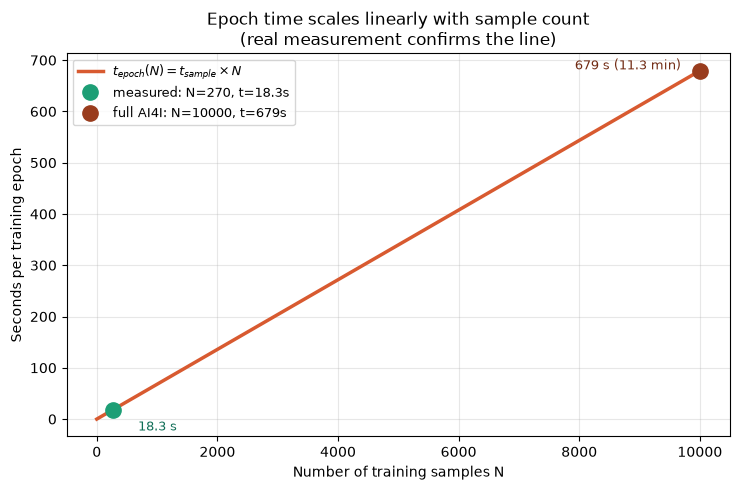
\includegraphics[width=0.75\textwidth]{figure/time_per_ep.png}
\caption{Measured PennyLane epoch time versus training-sample count at $n=8$ qubits (270 samples, 18.3\,s), extrapolated linearly to the full 10,000-row AI4I dataset (679\,s per epoch).}
\label{fig:time_per_ep}
\end{figure}

\begin{figure}[htbp]
\centering
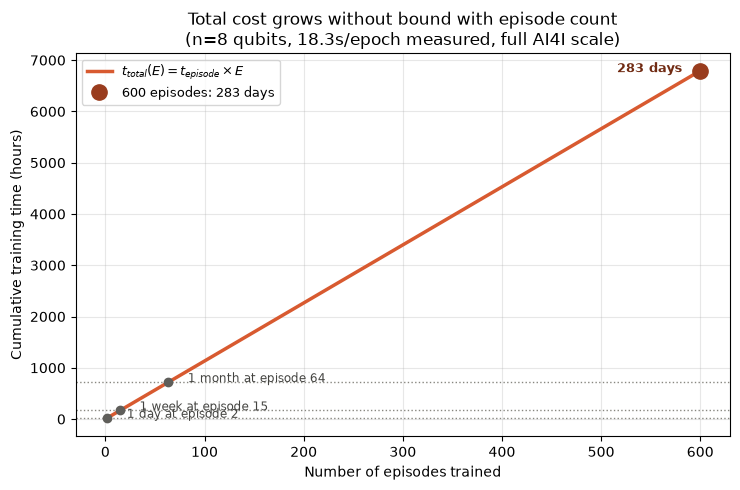
\includegraphics[width=0.75\textwidth]{figure/time_to.png}
\caption{Cumulative PennyLane training time versus episode count, built from the measured 18.3\,s/epoch figure at full-AI4I scale: 600 episodes (PPO's training length) would take approximately 283 days for a single agent.}
\label{fig:time_to_train}
\end{figure}

In practice, a result labelled ``simulate'' in this report (e.g. \Cref{tab:sim8g}) is generated entirely by the calibrated surrogate -- useful for isolating the effect of a single factor such as cost type quickly and cheaply, but not on its own a claim about the real circuit -- while a result labelled ``PennyLane'' (\Cref{tab:heart}) is the physically faithful case that the two-simulator design exists to make trainable in the first place.

\FloatBarrier
\subsubsection{Agent Design and States}
The scheduler is modelled formally as a Markov Decision Process, the tuple (S, A, P, R, $\gamma$) \citep{sutton2018reinforcement}. S is the sixteen-dimensional telemetry space described below; A is the five-action discrete space of \Cref{tab:actions}; P is the (unknown, backend-dependent) transition kernel induced by one epoch of circuit optimization under a chosen action; R is the scalar reward of Section~4.7.3; and $\gamma$ is the discount factor used by both agents to weight future epochs against the immediate one. Framing depth scheduling this way makes the problem amenable to standard policy-gradient and value-based RL methods without any quantum-specific modification to the algorithms themselves -- the quantum-specific part of the problem is entirely contained in how S, A, and R are computed from the circuit, not in how the agent is trained.

The state is a sixteen-dimensional telemetry vector summarizing the health of the circuit and its training dynamics; the most important components are listed in \Cref{tab:state}. The agent chooses among five discrete actions (\Cref{tab:actions}). Two agents are implemented and compared: a PPO actor-critic and a DQN value network. Both agents observe the identical state vector and act on the identical action space, so any difference in their behaviour reported in Section~6 is attributable to the learning algorithm rather than to a difference in what each agent is allowed to see or do.

\begin{table}[htbp]
\centering
\caption{Groups of the 16-dimensional MDP state vector (STATE\_DIM = 16).}
\label{tab:state}
\begin{tabular}{|p{3cm}|p{10cm}|}
\hline
\textbf{Group} & \textbf{Representative features} \\
\hline
Gradient health & spatial gradient variance, gradient norm, near-zero-gradient ratio \\
Training dynamics & training loss, validation loss, change in loss ($\Delta$loss) \\
Architecture & current depth, number of entangling gates, remaining depth budget \\
Diagnosis (Section~4.4.1) & solved/converged, local-minimum, dead-layer, ambiguous, and true-barren-plateau flags \\
Derived & relative weak-layer indicator (rel\_weak) and other normalized ratios \\
\hline
\end{tabular}
\end{table}

\begin{table}[htbp]
\centering
\caption{Action space (N\_ACTIONS = 5).}
\label{tab:actions}
\begin{tabular}{|p{4.5cm}|p{8.5cm}|}
\hline
\textbf{Action} & \textbf{Effect} \\
\hline
keep & Hold the current architecture and continue training. \\
add\_layer & Append a new parameterized layer (subject to the mask window). \\
propose\_prune\_layer & Soft-mask a layer for possible removal. \\
stop\_growth & Freeze the architecture for the remainder of training. \\
propose\_reduce\_entanglement & Reduce the entangling strength among gates. \\
\hline
\end{tabular}
\end{table}

\subsubsection{Reward System}
The reward combines several terms that trade off gradient health, loss improvement, and resource use. The weights actually used are given in \Cref{tab:reward}. An important and honestly-reported consequence of these weights is that the loss-improvement term (weight 5.0) dominates the gradient-variance term (weight 0.5): across the regimes reported in Section~6, this means the agent chiefly learns to optimize loss under a resource constraint rather than to avoid barren plateaus directly, and at the qubit counts evaluated here a clearly separable plateau-avoidance signal -- where growing depth is driven by low gradient variance rather than by loss alone -- has not been isolated; whether one would emerge under a local cost at a larger, currently out-of-scope qubit count (Section~1.6) is accordingly left as an open question rather than a demonstrated result.

\begin{table}[htbp]
\centering
\caption{Reward-term weights.}
\label{tab:reward}
\begin{tabular}{|p{1.5cm}|p{1.8cm}|p{9.5cm}|}
\hline
\textbf{Term} & \textbf{Weight} & \textbf{Meaning} \\
\hline
w1 & 0.5 & gradient-variance health \\
w2 & 5.0 & improvement in loss ($\Delta$loss) -- dominant term \\
w3 & 0.05 & depth / resource penalty \\
w4 & 0.02 & entangling-gate penalty \\
w5 & 1.0 & commit bonus for accepted mutations \\
w6 & 0.5 & rollback / stability shaping \\
\hline
\end{tabular}
\end{table}

\subsubsection{RL Algorithm and Training Strategy}
Two standard algorithms are used without exotic modifications. PPO \citep{schulman2017proximal} is a clipped-objective actor-critic that updates the policy conservatively; it is trained for 600 episodes. \Cref{fig:ppo_arch} shows its architecture: a shared two-layer, 128-unit MLP body (Tanh) feeds a masked 5-logit policy head and a scalar value head; each update computes a normalized GAE advantage from the stored rollout and applies the clipped surrogate objective (probability ratio clipped to $\pm20\%$) over 10 epochs of minibatch-64 backpropagation. DQN \citep{mnih2015human} is a value-based method with a target network and experience replay; it is trained for 1000 episodes. \Cref{fig:dqn_arch} shows its architecture: an online Q-network (the same two-layer, 128-unit body, ReLU instead of Tanh) outputs five Q-values; invalid actions are masked to $-\infty$ \emph{after} the network rather than inside it, transitions are pushed to a 50k-capacity replay buffer and sampled in minibatches of 64, and the target is computed Double-DQN style -- the online network selects the action, the target network evaluates it -- before a smooth-L1 TD loss updates the online network. Both use action masking so that invalid mutations (for example adding beyond the depth cap) are never selected. Proposed mutations are evaluated inside a soft-mask window and are either committed if they improve a peak-loss criterion or rolled back otherwise, which gives the agent a safe way to explore architecture changes without permanently damaging the model.

\begin{figure}[htbp]
\centering
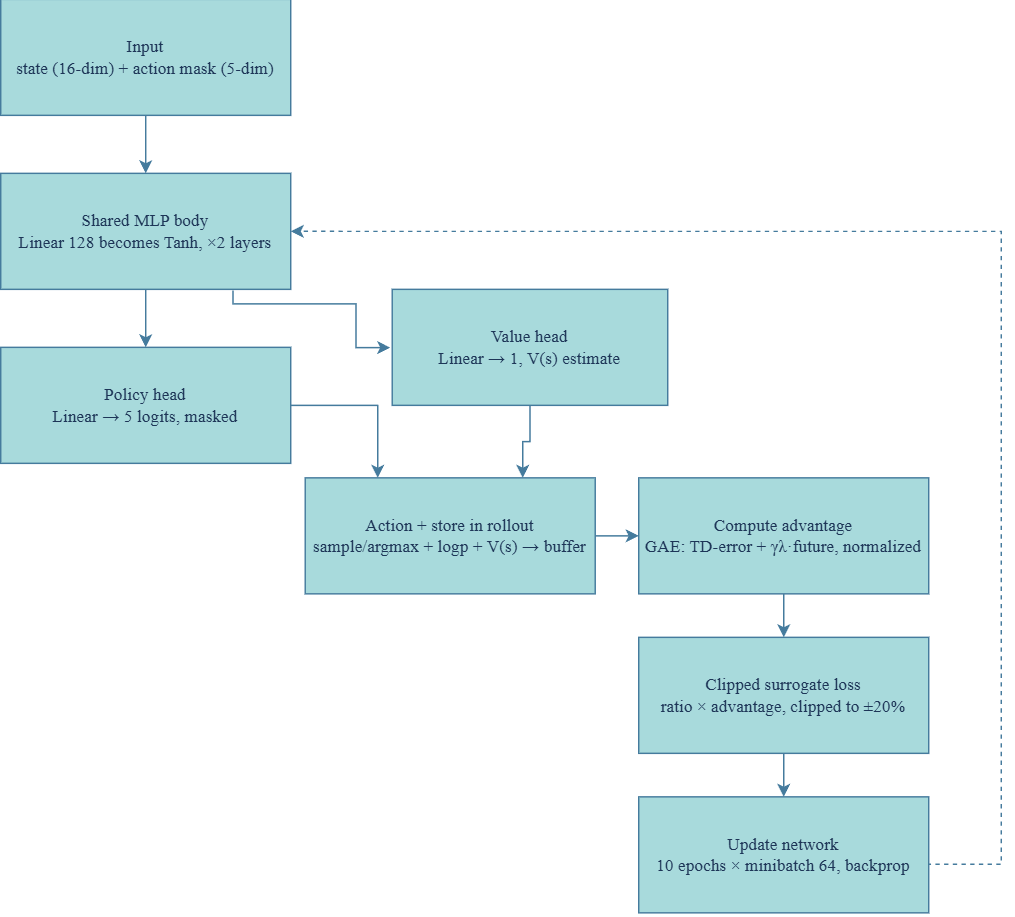
\includegraphics[width=0.7\textwidth]{figure/PPO.drawio.png}
\caption{PPO network architecture and update loop: shared MLP body, masked policy head and value head, GAE advantage estimation, and the clipped surrogate objective.}
\label{fig:ppo_arch}
\end{figure}

\begin{figure}[htbp]
\centering
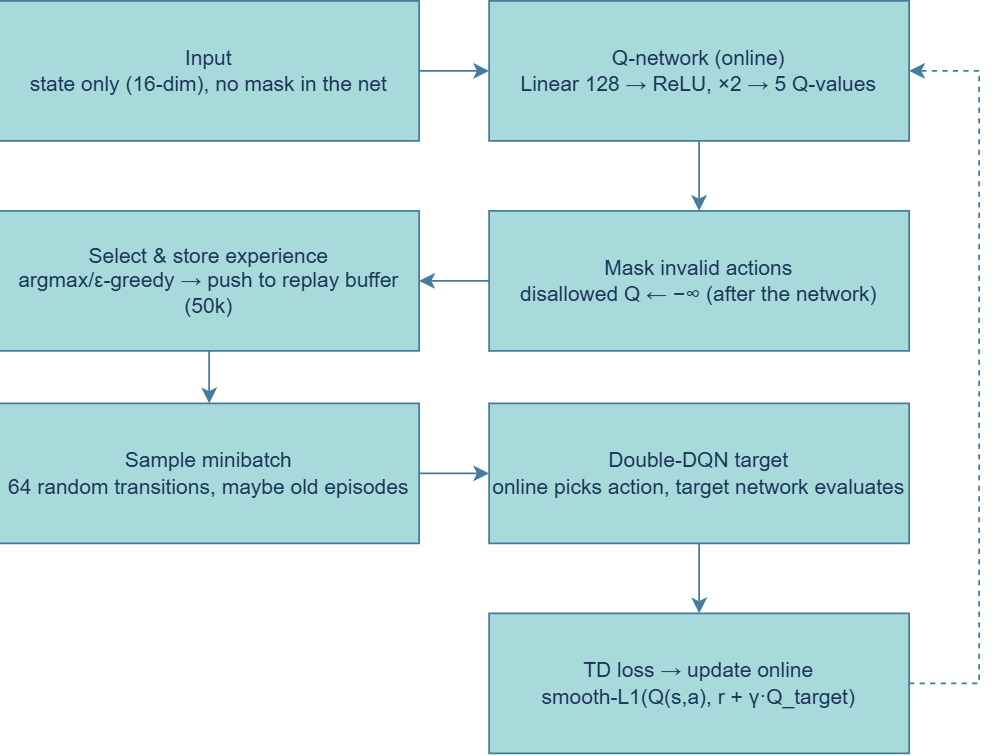
\includegraphics[width=0.7\textwidth]{figure/DQN.drawio.png}
\caption{DQN network architecture and update loop: online Q-network, post-hoc action masking, replay-buffer sampling, and the Double-DQN target used for the smooth-L1 TD update.}
\label{fig:dqn_arch}
\end{figure}

\FloatBarrier
\subsubsection{Static Baseline Schedulers}
The two static baselines that every table in Section~6 compares the learned agents against are themselves rule-based decision trees over the same telemetry and the same offline, calibrated threshold $\tau$ from the Stage~1C risk table (Section~4.7.1), not free parameters left unspecified. \Cref{fig:rule_baseline} shows the hand-tuned \textbf{Rule} scheduler: in a fixed priority order, it prunes a layer diagnosed as dead, else reduces entanglement if the gradient norm signals a global barren-plateau risk, else adds a layer while the circuit is still shallow (depth $<6$) and loss is stable, else stops growth once depth reaches 6, holding the architecture otherwise. \Cref{fig:greedy_baseline} shows the \textbf{Greedy} heuristic, the same four-branch structure with different, more aggressive thresholds: a layer is pruned once it contributes less than 15\% of the mean layer weight, entanglement is reduced once the near-zero-gradient ratio (\Cref{tab:state}) reaches 0.4, growth stops once the gradient variance has both hit its calibrated floor and fallen to or below $\tau$, and a layer is added whenever variance exceeds three times $\tau$. Both baselines are deterministic and receive no training; the only difference between them and the learned agents above is that their mapping from telemetry to action is hand-specified rather than learned from the reward of \Cref{tab:reward}.

\begin{figure}[htbp]
\centering
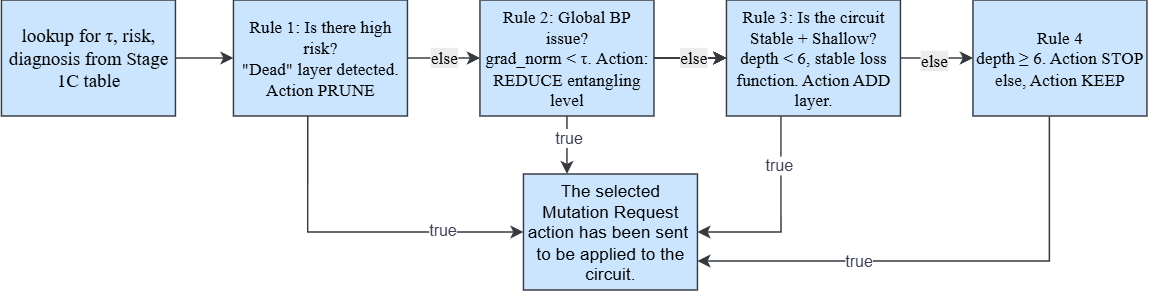
\includegraphics[width=1\textwidth]{figure/Rule.drawio.png}
\caption{Decision logic of the hand-tuned Rule baseline: a fixed priority order over dead-layer pruning, global-BP entanglement reduction, growth, and a depth-6 stop condition.}
\label{fig:rule_baseline}
\end{figure}

\begin{figure}[htbp]
\centering
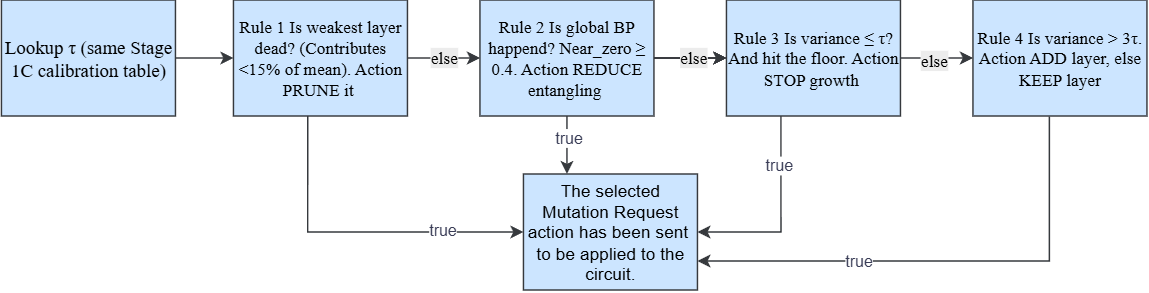
\includegraphics[width=1\textwidth]{figure/greedy.drawio.png}
\caption{Decision logic of the Greedy baseline: the same four-branch structure as the Rule baseline, with different thresholds (15\% weakest-layer contribution, 0.4 near-zero-gradient ratio, and a variance-relative-to-$\tau$ stop/grow condition).}
\label{fig:greedy_baseline}
\end{figure}

Algorithm~1 formalizes the per-epoch loop that both agents interact with, independently of which physics backend (simulate or PennyLane) is behind it. The commit/rollback guard is what allows the agent to propose a structural change to the circuit without risking the run: a proposal is only made permanent if it improves the tracked peak-loss criterion, and is otherwise reverted before the next epoch begins.

\begin{algorithm}[h]
\caption{One deployment/training epoch under the agent-controlled environment}
\label{alg:epoch}
\begin{algorithmic}[1]
\State \textbf{Input:} circuit at depth $d$, telemetry state $s_t$, peak-loss tracker $L^\star$
\State $a_t \gets \pi(s_t)$ \Comment{agent selects one of the five actions (\Cref{tab:actions})}
\If{$a_t$ proposes a structural change (add / prune / reduce-entanglement)}
    \State apply $a_t$ inside a soft-mask window (change not yet permanent)
\EndIf
\State run one epoch of parameter optimization on the (possibly masked) circuit
\State observe new loss $L_t$, gradient variance, and the rest of $s_{t+1}$
\If{$a_t$ proposed a structural change}
    \If{$L_t$ improves on $L^\star$}
        \State \textbf{commit}: make the change permanent; $L^\star \gets L_t$
    \Else
        \State \textbf{rollback}: revert to the pre-mutation architecture
    \EndIf
\EndIf
\State compute reward $r_t$ from $s_{t+1}$ (\Cref{tab:reward}) and return $(s_{t+1}, r_t)$
\end{algorithmic}
\end{algorithm}

The agent is trained entirely on the calibrated surrogate, where an episode corresponds to a full training run of the circuit under the agent's decisions. The learned policy is then deployed on the PennyLane statevector backend for 40 epochs, which is where all reported metrics are computed. During development, configurations were run with three random seeds on the AI4I dataset to characterize seed variance; the scheduler-comparison tables presented in Section~6 are run single-seed, always against the same two static baselines: a hand-tuned rule-based scheduler and a greedy heuristic.

\FloatBarrier
\subsubsection{Implementation Details}
The system is implemented in Python. Quantum circuits use PennyLane with the default statevector device and backpropagation gradients; the RL agents use PyTorch. The hardware-efficient ansatz is defined exactly once (single source of truth) and reused by the barren-plateau measurement stage and the deployment backend, so any ansatz change propagates automatically. Because full-simulator training would be prohibitively slow even at the project's 8-qubit scope (Section~1.6), the surrogate reduces RL training to roughly half an hour per agent.

\subsection{Ethical Considerations}

\subsubsection{Data Sensitivity}
Several datasets are sensitive: German Credit concerns financial creditworthiness and the medical datasets concern health status. The project uses these strictly as research benchmarks and does not deploy any model for real decisions, so the risk of biased or harmful predictions in practice does not arise here; nonetheless, class balancing and consistent preprocessing are applied so that reported accuracy is not inflated by imbalance. Because all experiments run on a simulator, there is no physical-hardware safety risk.

\subsubsection{Reproducibility and Data Honesty}
The project's overriding ethical commitment is data honesty -- every reported number is reproducible from a committed log, single-seed results are labelled as such, and unsupported performance claims were removed.

